\section{Prediction for unassociated sources in 3FGL and comparison with 4FGL}
\lb{sec:3FGLprediction}


In this section we use of the selected algorithms from the previous section to predict classes for the unassociated sources in the 3FGL. 
We then use the associations, which exist for some of these sources in the 4FGL, to check the accuracy of our methods on the unassociated data.  A total of 286 such sources were identified. These contain 20 pulsars.
\dima{The 286 sources contain only pulsars and AGNs or other sources as well. If there are other sources, it is not clear how do we do comparison with the predicted classes.}

%\subsection{Unassociated sources in 3FGL with associations in 4FGL}
%There were a total of 286 sources without associations in 3FGL but associations in 4FGL. We trained our algorithms on the entire set of associated data from the 3FGL, and then tested our algorithms on these 286 sources. The probabilistic version is discussed in the next section.  \\
Accuracy of the prediction of the source classes compared to the 4FGL classes for RF and BDT algorithms is shown in Figure \ref{fig:RF_BDT_4FGL_accuracy}.
The accuracy of the RF algorithm increases with the depth of the trees and the number of trees in the forest
up to maximal depth of about 15 and 200 trees in the forest, after that the accuracy stays constant.
For the BDT, the accuracy decreases for depth larger than about 10, it does not depend on the number of trees above XXX trees.
\dima{We should plot BDT with fewer numbers of trees, e.g., 5, 10, 20, 50, it looks like soon after 20 trees BDT converges and accuracy does not change for larger number of trees.}

%Here we can see how Random Forests and BDT accuracies depend on the complexity of the network. Random Forests follow the same pattern as seen with the associated data with greater complexity allowing for a higher accuracy of the sources. Boosted Decision Trees also lower the accuracy as the maximum depth increases, although there seem to be certain points where the accuracy suddenly rises up. As seen with the training data, here also the BDT models converge to an accuracy value which is only dependent on the number of trees\\

\begin{figure}[h]
%\centerin
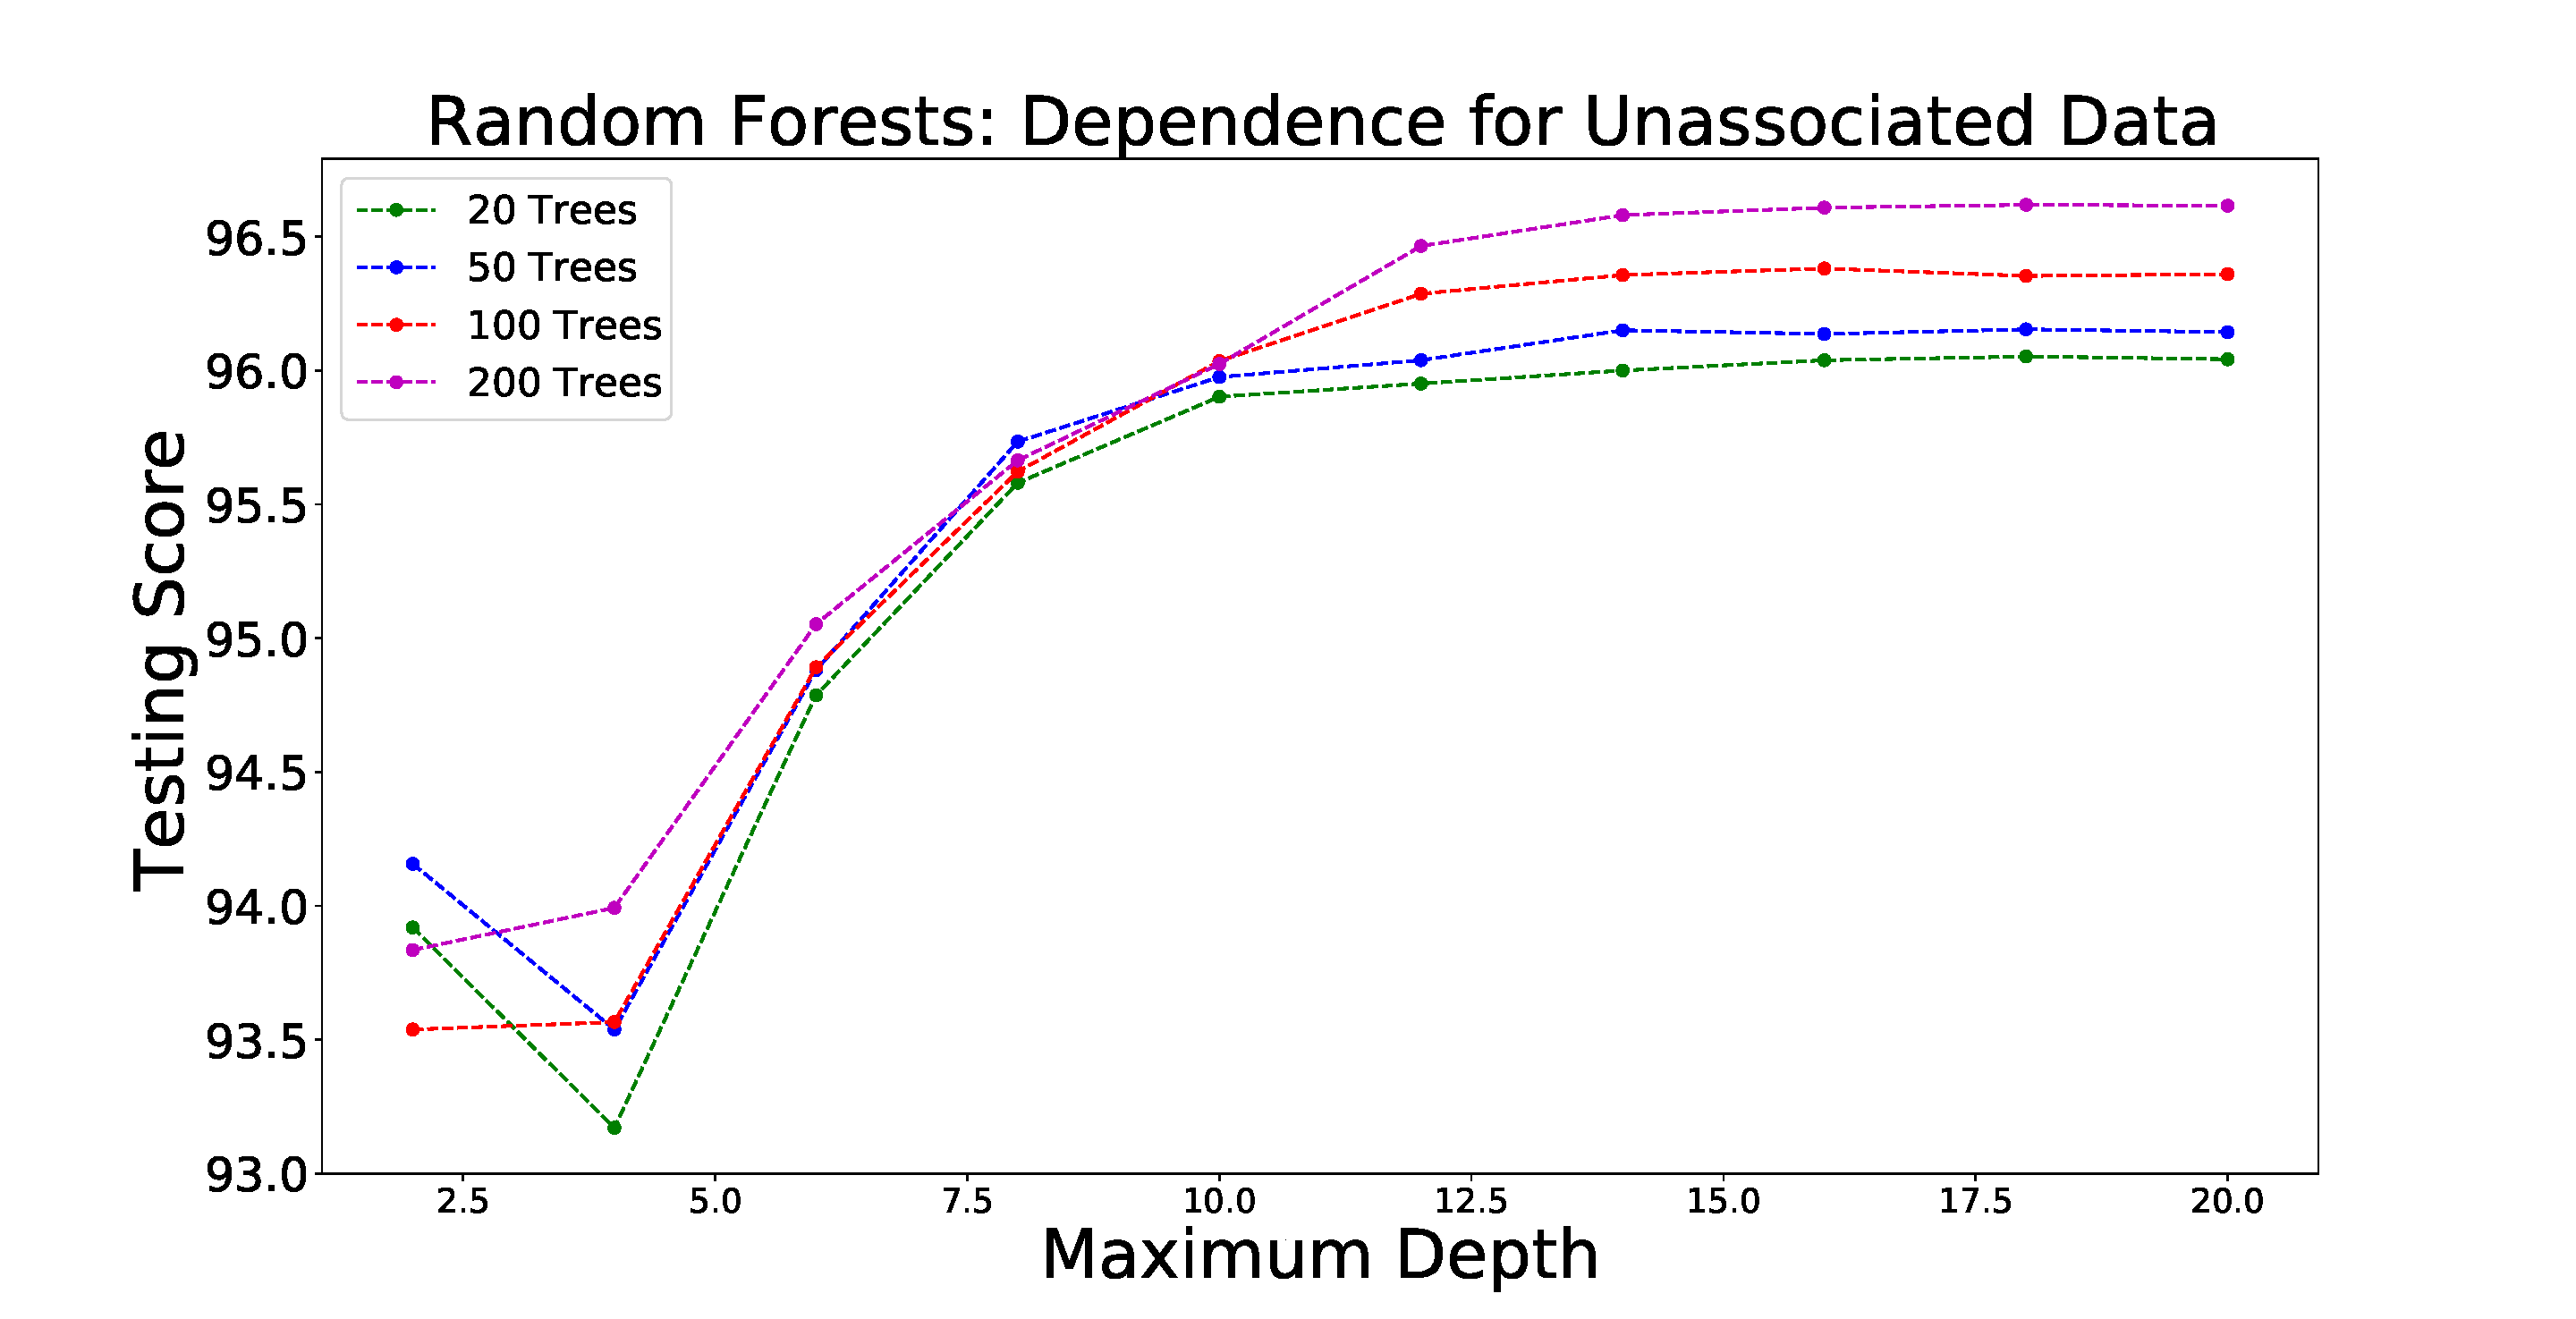
\includegraphics[width=\twopicsp\textwidth]{plots/unassoc2.pdf}
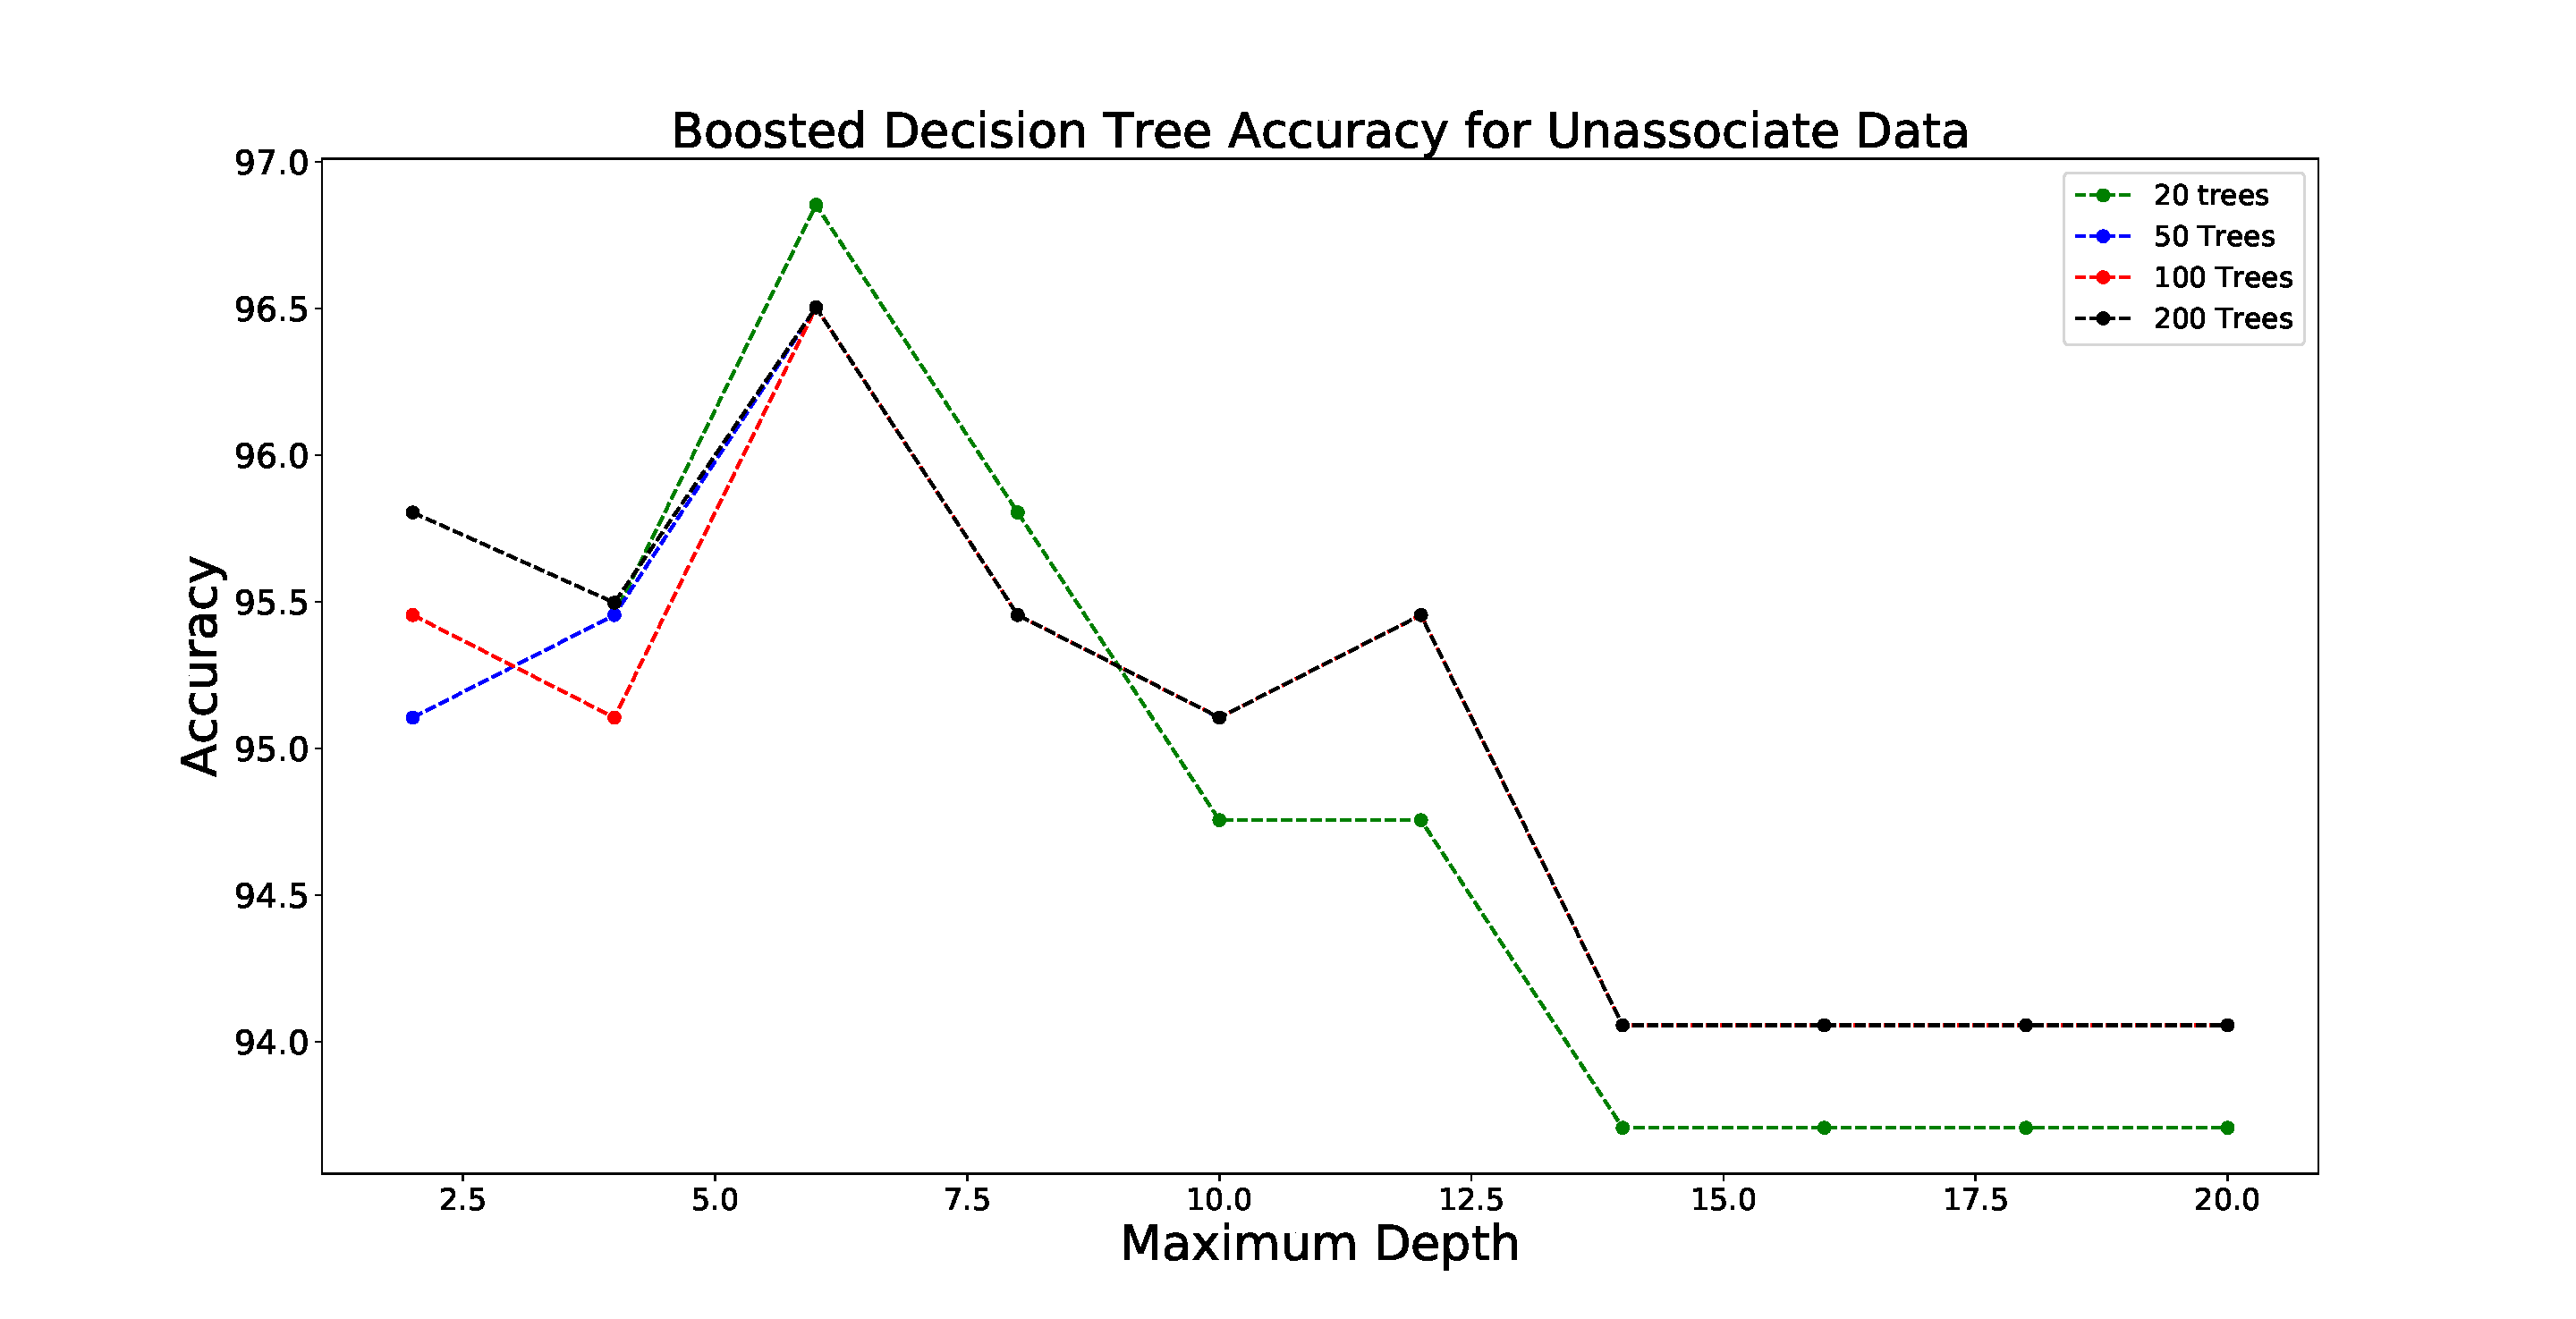
\includegraphics[width=\twopicsp\textwidth]{plots/unassoc_complex.pdf}
\caption{RF and BDT accuracy of class prediction for unassociated 3FGL sources compared to associations in the 4FGL}
\label{fig:RF_BDT_4FGL_accuracy}
\end{figure}

%Neural Networks, unlike random forests are susceptible to overtraining, as can be seen in the figures below. Increase the complexity of the network leads to a slight decrease in accuracy. This is seen for both single hidden layer networks and two hidden layer networks where the first layer has 5 neurons. Here Adam slightly outperforms lbfgs, especially when different activation functions are used. \\
Accuracies for NN and LR algorithms are presented in Figure \ref{fig:NN_LR_4FGL_accuracy}.
\dima{As in the previous section, I think we should plot NN for neurons from 2 (or even 1) to about 20, although it really makes sense to plot only up to 10 neurons.}
An interesting result is found for LR case where the SAGA solver performs better than the L-BFGS, which is different from the results obtained with the training dataset. This is likely because the SAGA solver allows for a more general model than the L-BFGS one. \dima{Why?}

\begin{figure}[h]
%\centerin
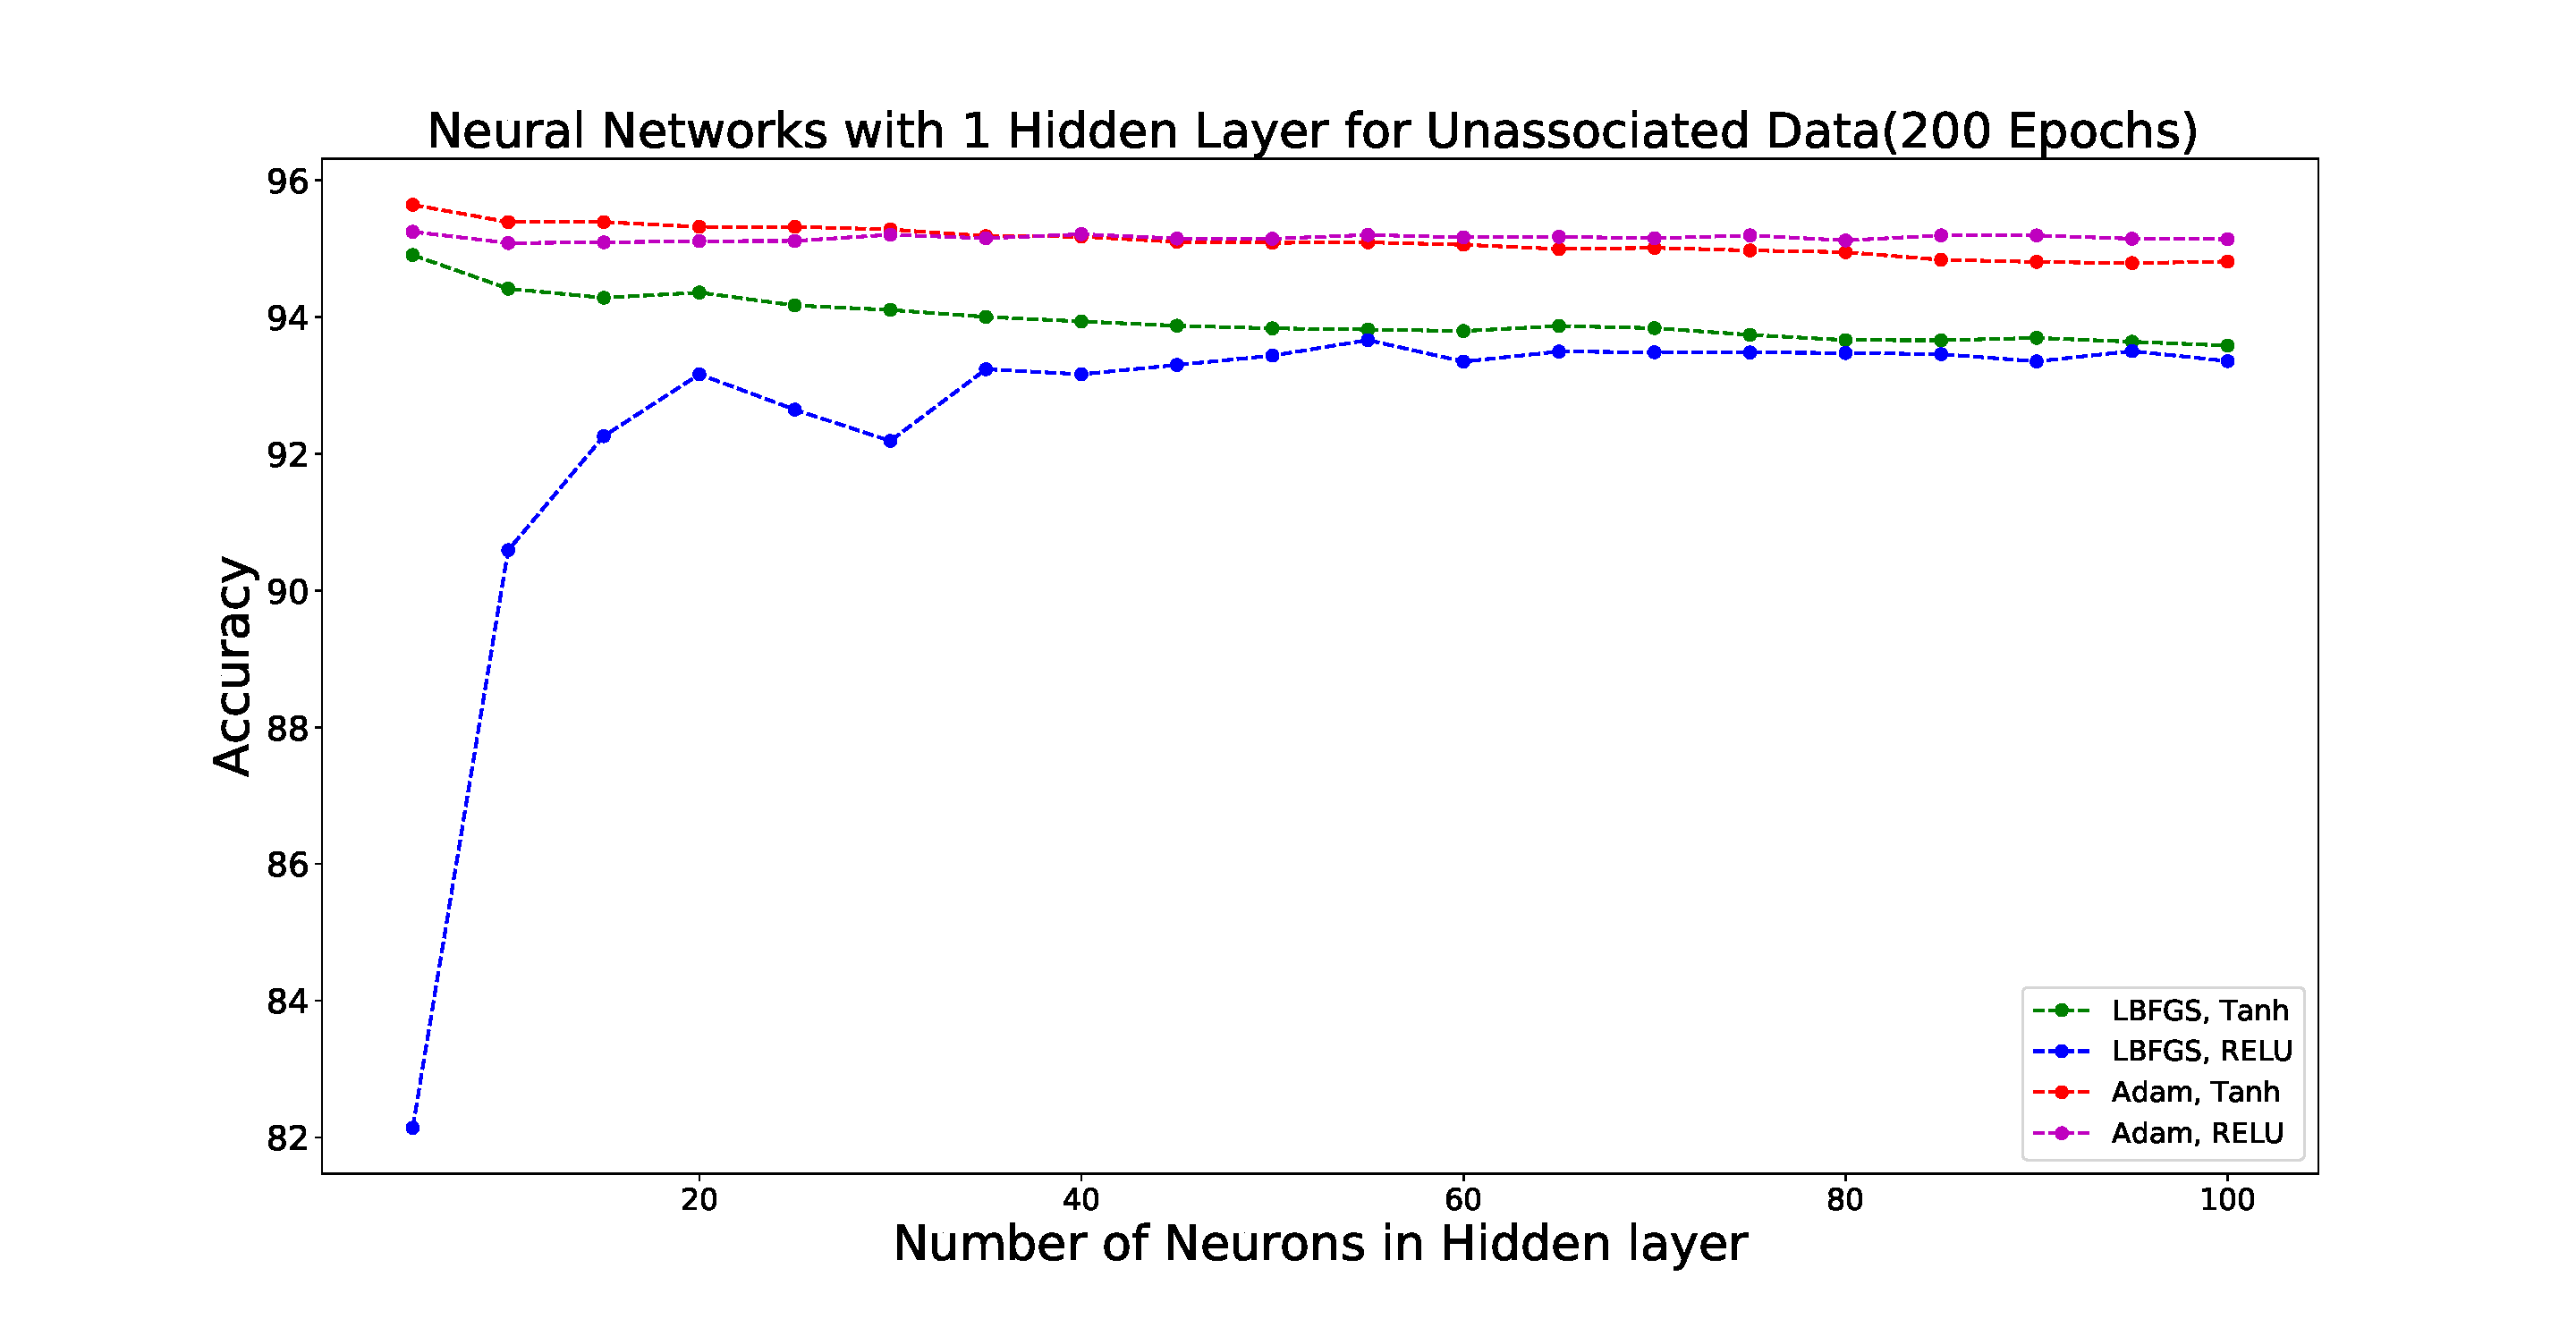
\includegraphics[width=\twopicsp\textwidth]{plots/neurons4.pdf}
%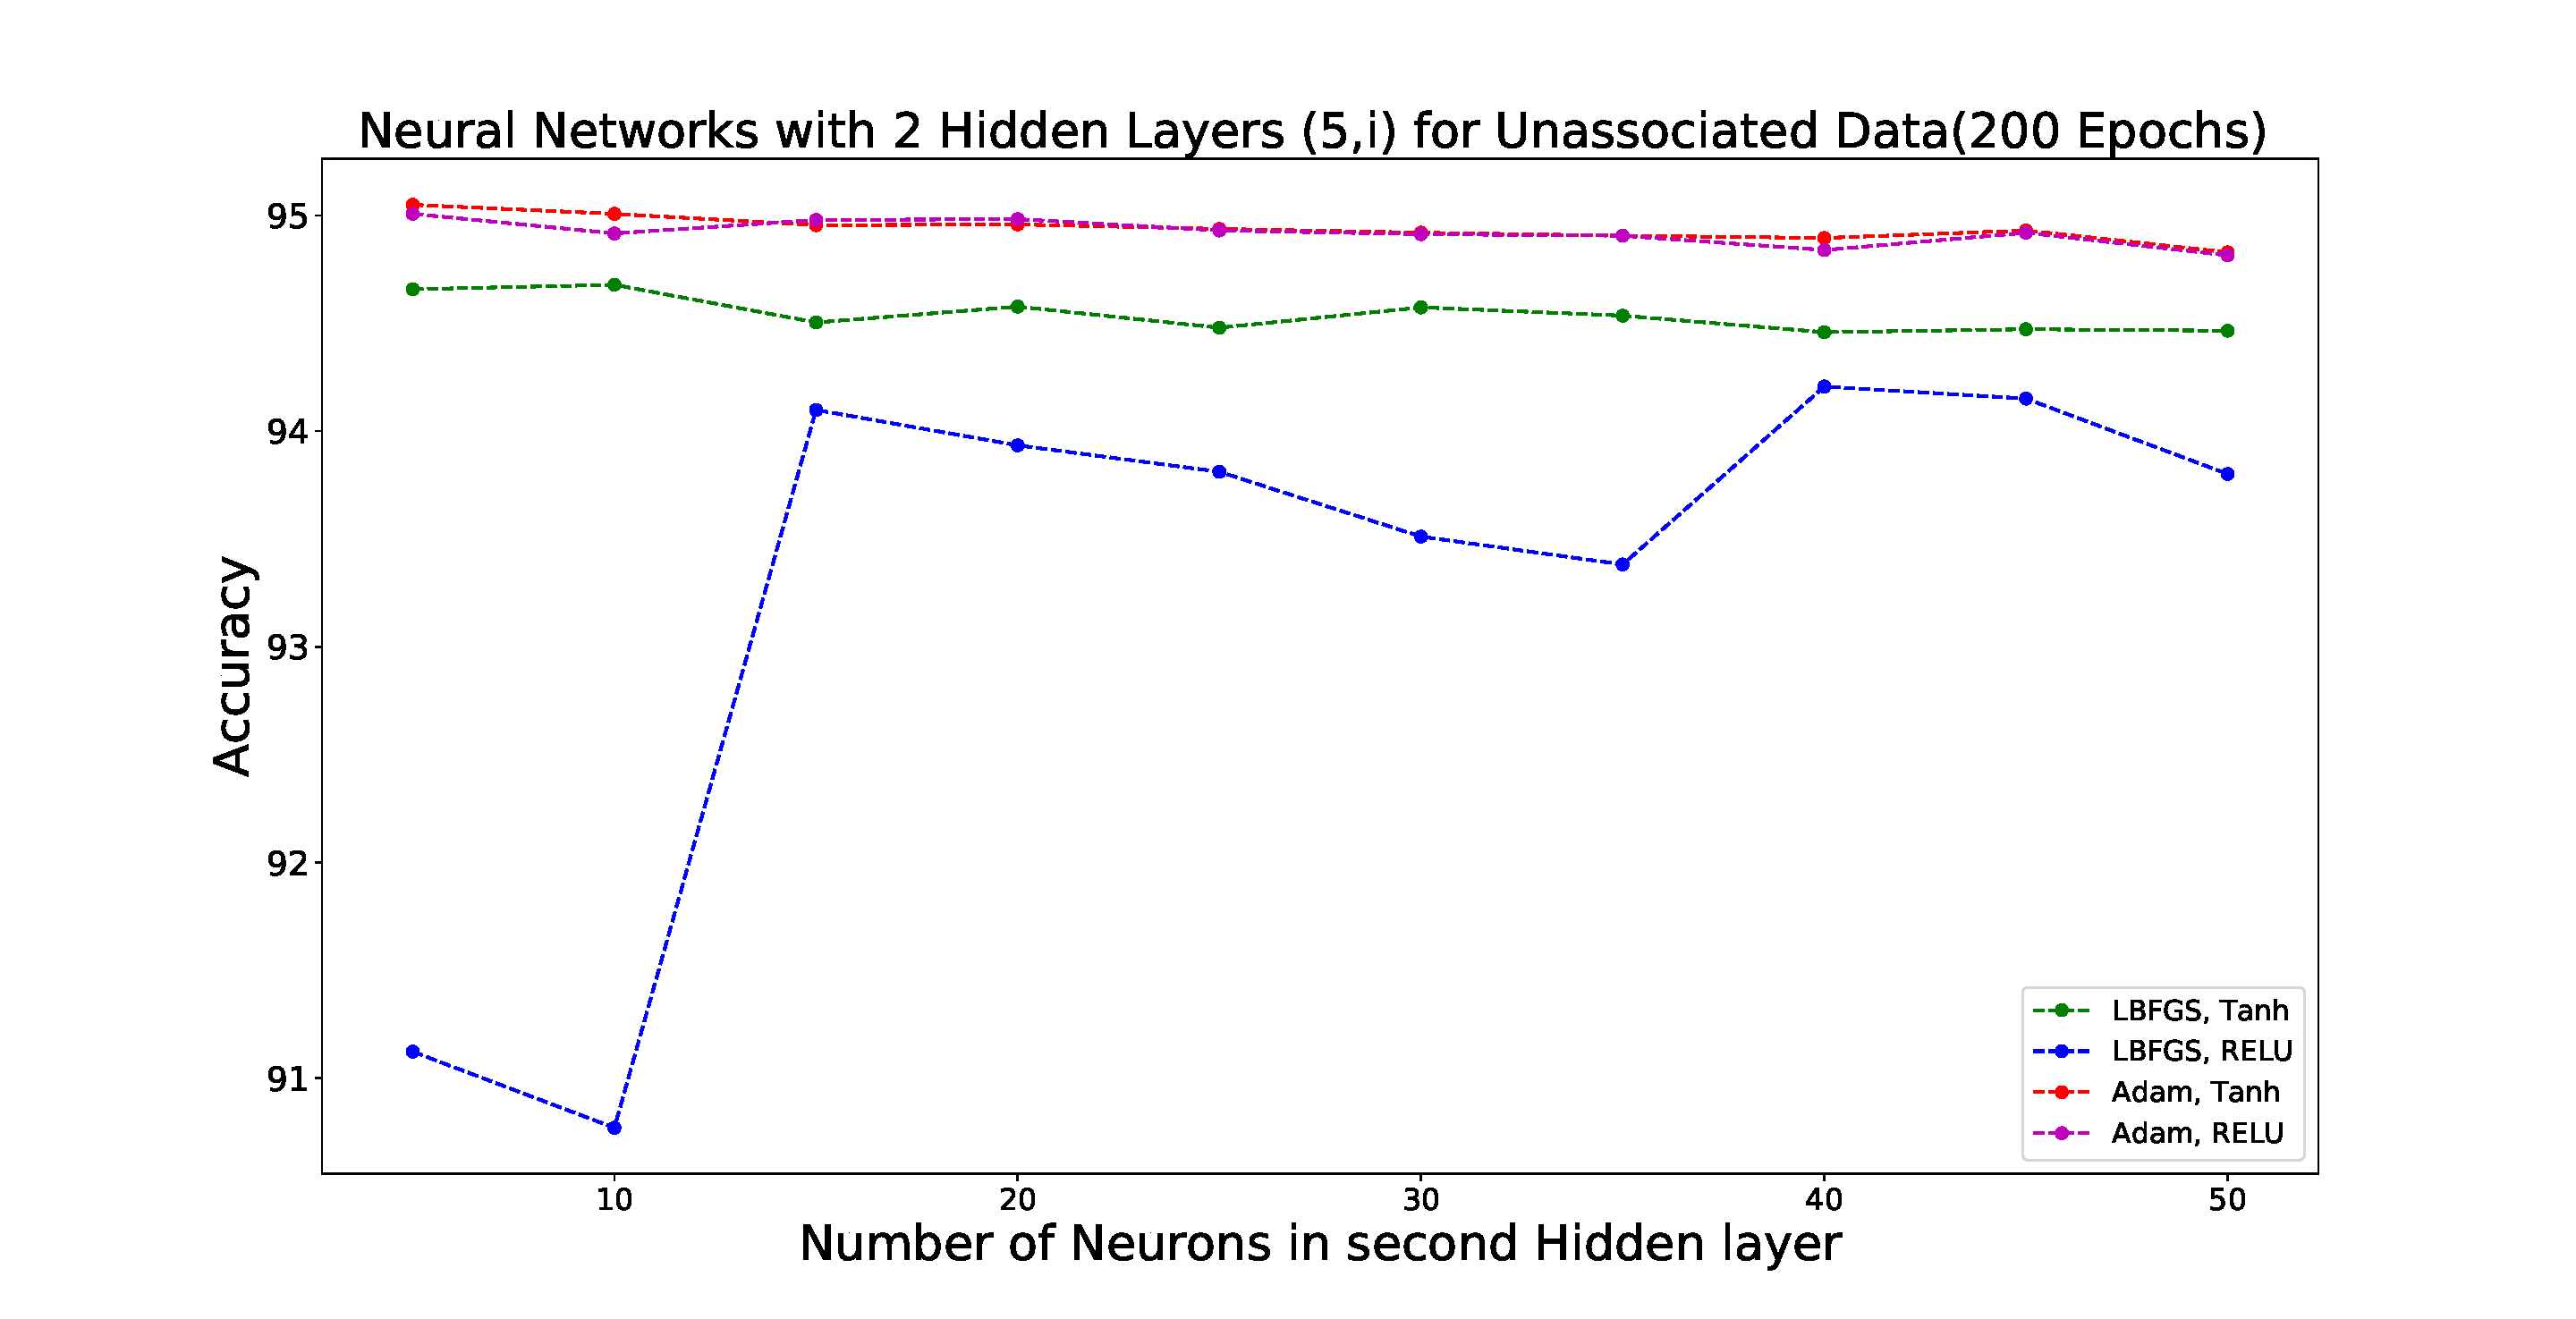
\includegraphics[width=\twopicsp\textwidth]{plots/neurons5.pdf}
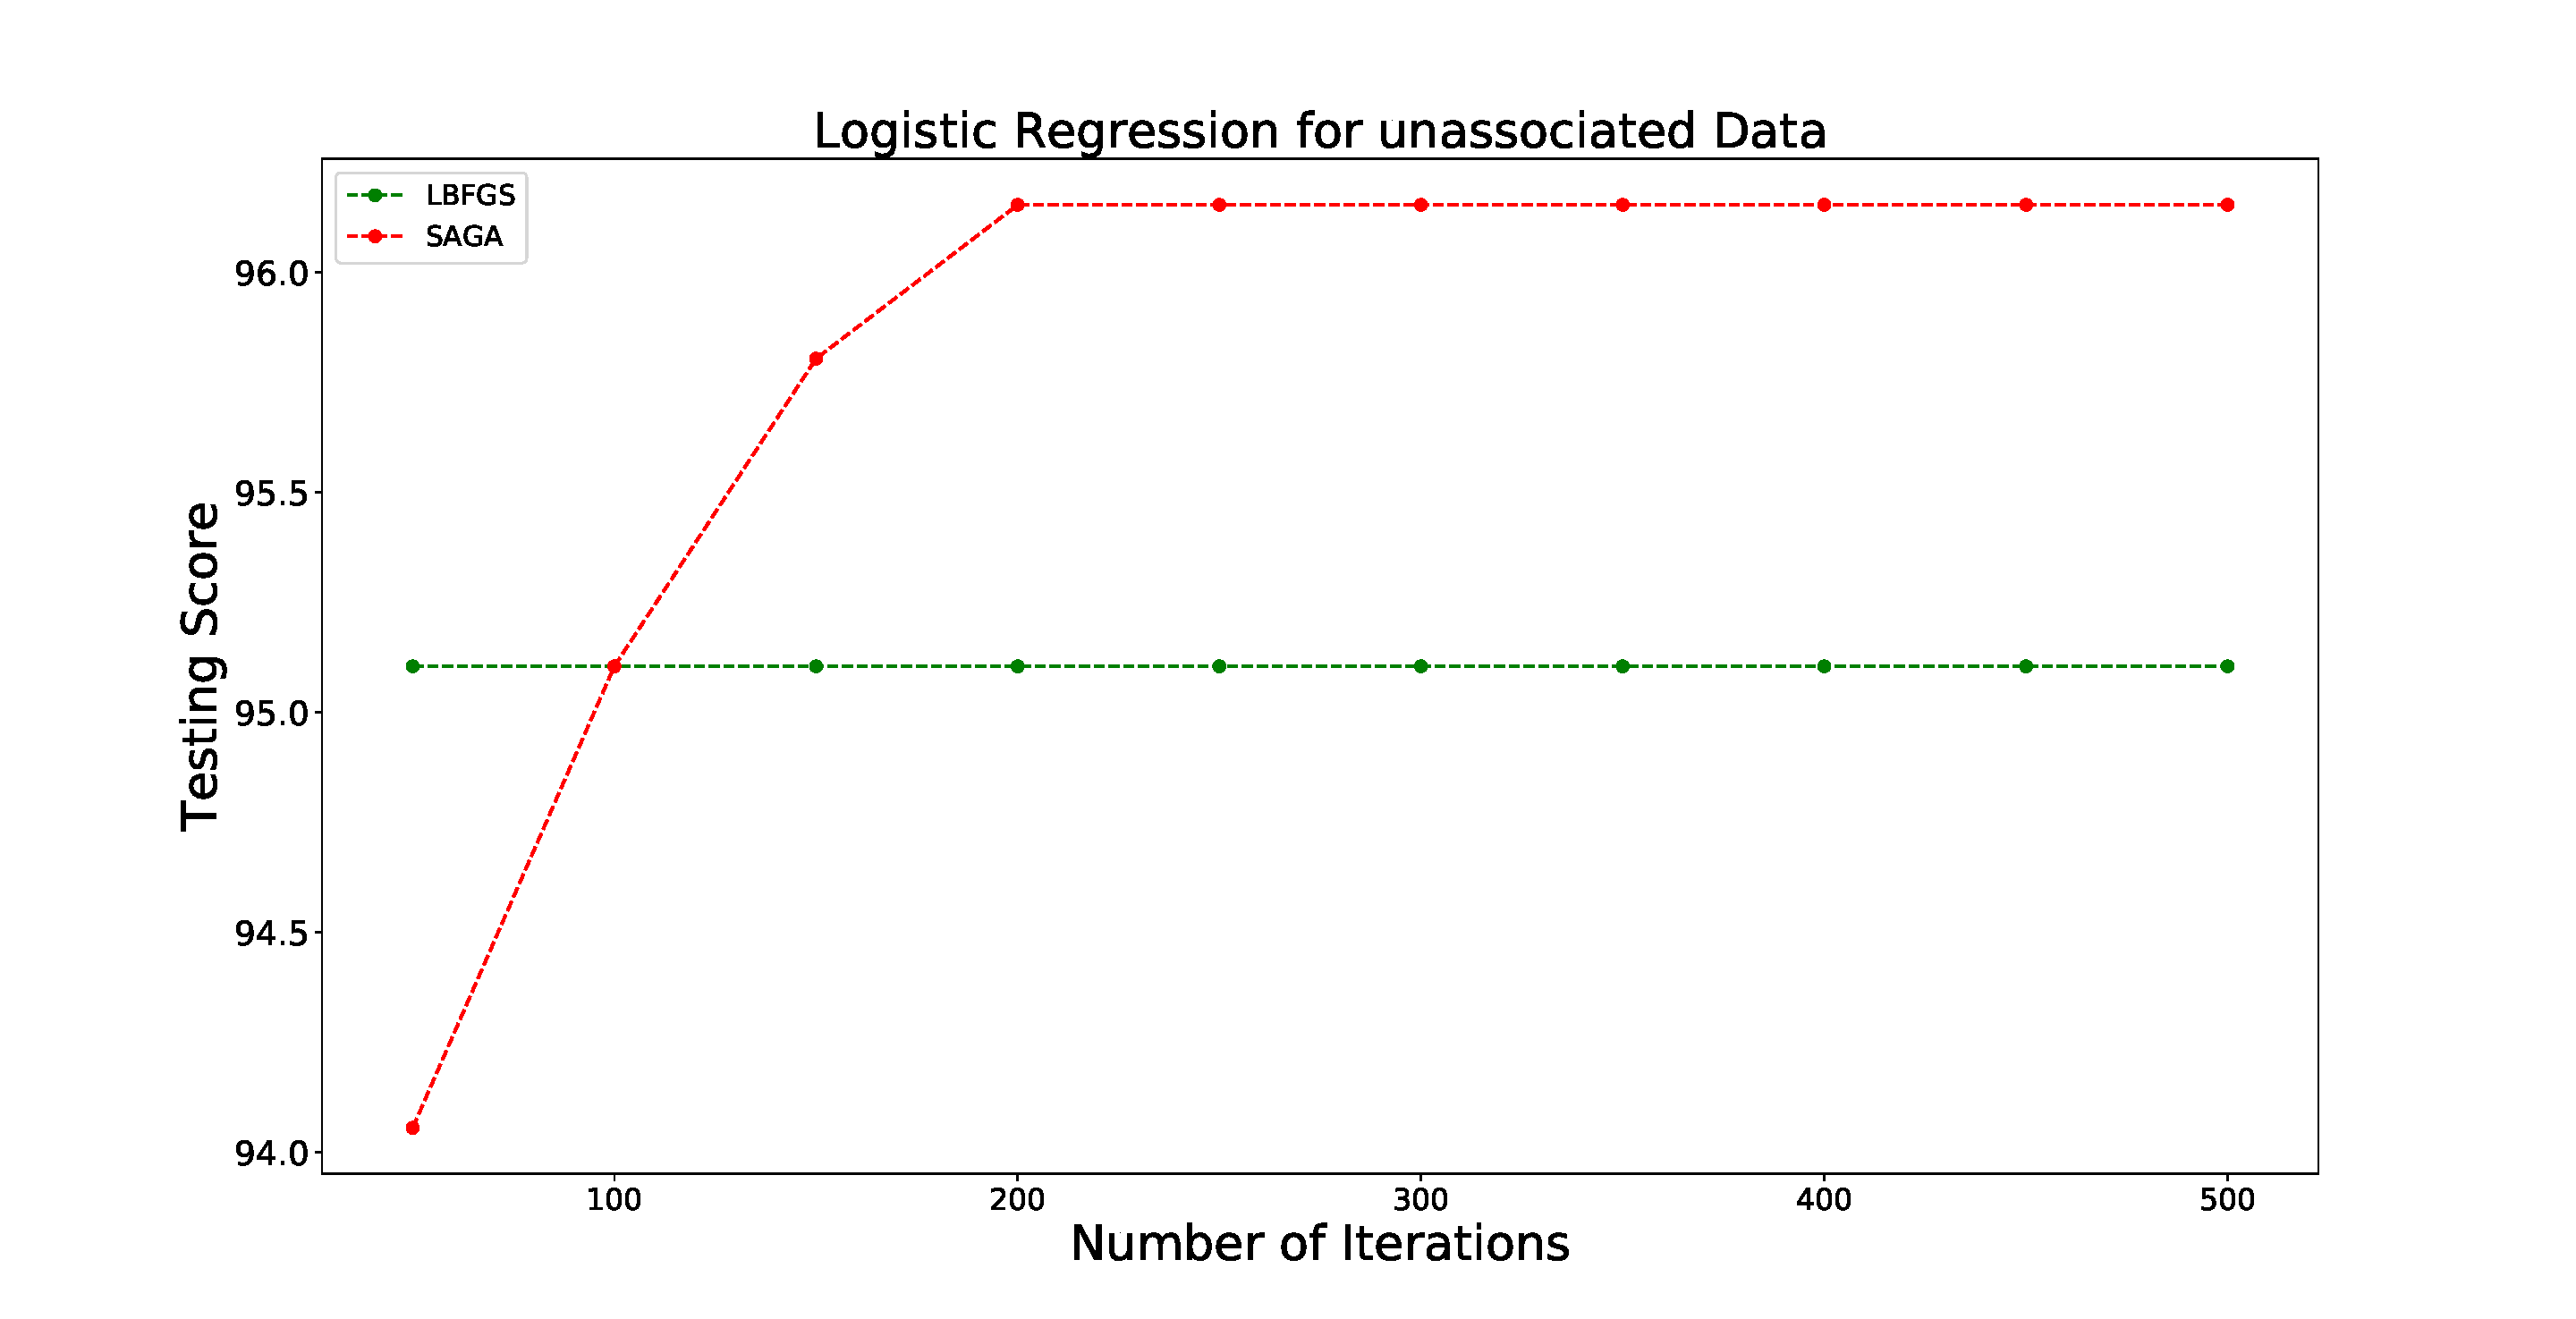
\includegraphics[width=\twopicsp\textwidth]{plots/solver_unass.pdf}
\caption{Logistic Regression and Neural Network accuracies}
\label{fig:NN_LR_4FGL_accuracy}
\end{figure}

Finally, we chose our best models to create a probabilistic catalog. The following were the accuracies we found for 1000 runs using the best models we had.
\dima{I think we should select the models based on the test data-set for the 3FGL in the previous section, rather than on the comparison with 4FGL. The conceptual reason is that we should choose the algorithms before we apply them to the real data, 
otherwise there is a danger of overfitting, which we cannot evaluate. Table \ref{tab:selected_algs} should be at the end of Section 3, where we should also include a discussion on which algorithms we choose for predictions in sections 4 and 5.}



\begin{table}[!h]
    \tiny
    \centering
    \renewcommand{\tabcolsep}{1mm}
\renewcommand{\arraystretch}{1.5}

    \begin{tabular}{|c|c|c|}
    \hline
    Algorithm&Parameters & Accuracy\\
    \hline
    RF& 200 trees, max depth 15  & 96.55   \\
    \hline
    NN & 200 epochs, 1 hidden layer, 5 neurons &  95.58 \\
    \hline %\midrule   -> aakash do you mean this?
    BDT & 50 trees, max depth 10    &   95.27  \\
%    \hline %\midrule   -> aakash do you mean this?
%    BDT & 200 trees, max depth 2    &   95.8  \\
    \hline
    LR & SAGA solver, 200 iterations & 95.45 \\
    \hline
     
    \end{tabular}

    \caption{Testing Accuracy of the 4 selected algorithms on 3FGL unassociated data.}
    \label{tab:selected_algs}
\end{table}

%As can be seen above, the best accuracies were found with less complicated models, which allowed bias to be low. The models were complicated enough to neither under, nor overtrain.

\subsection{3FGL Probabilistic classification} 

\begin{figure}[h]
%\centerin
<<<<<<< HEAD
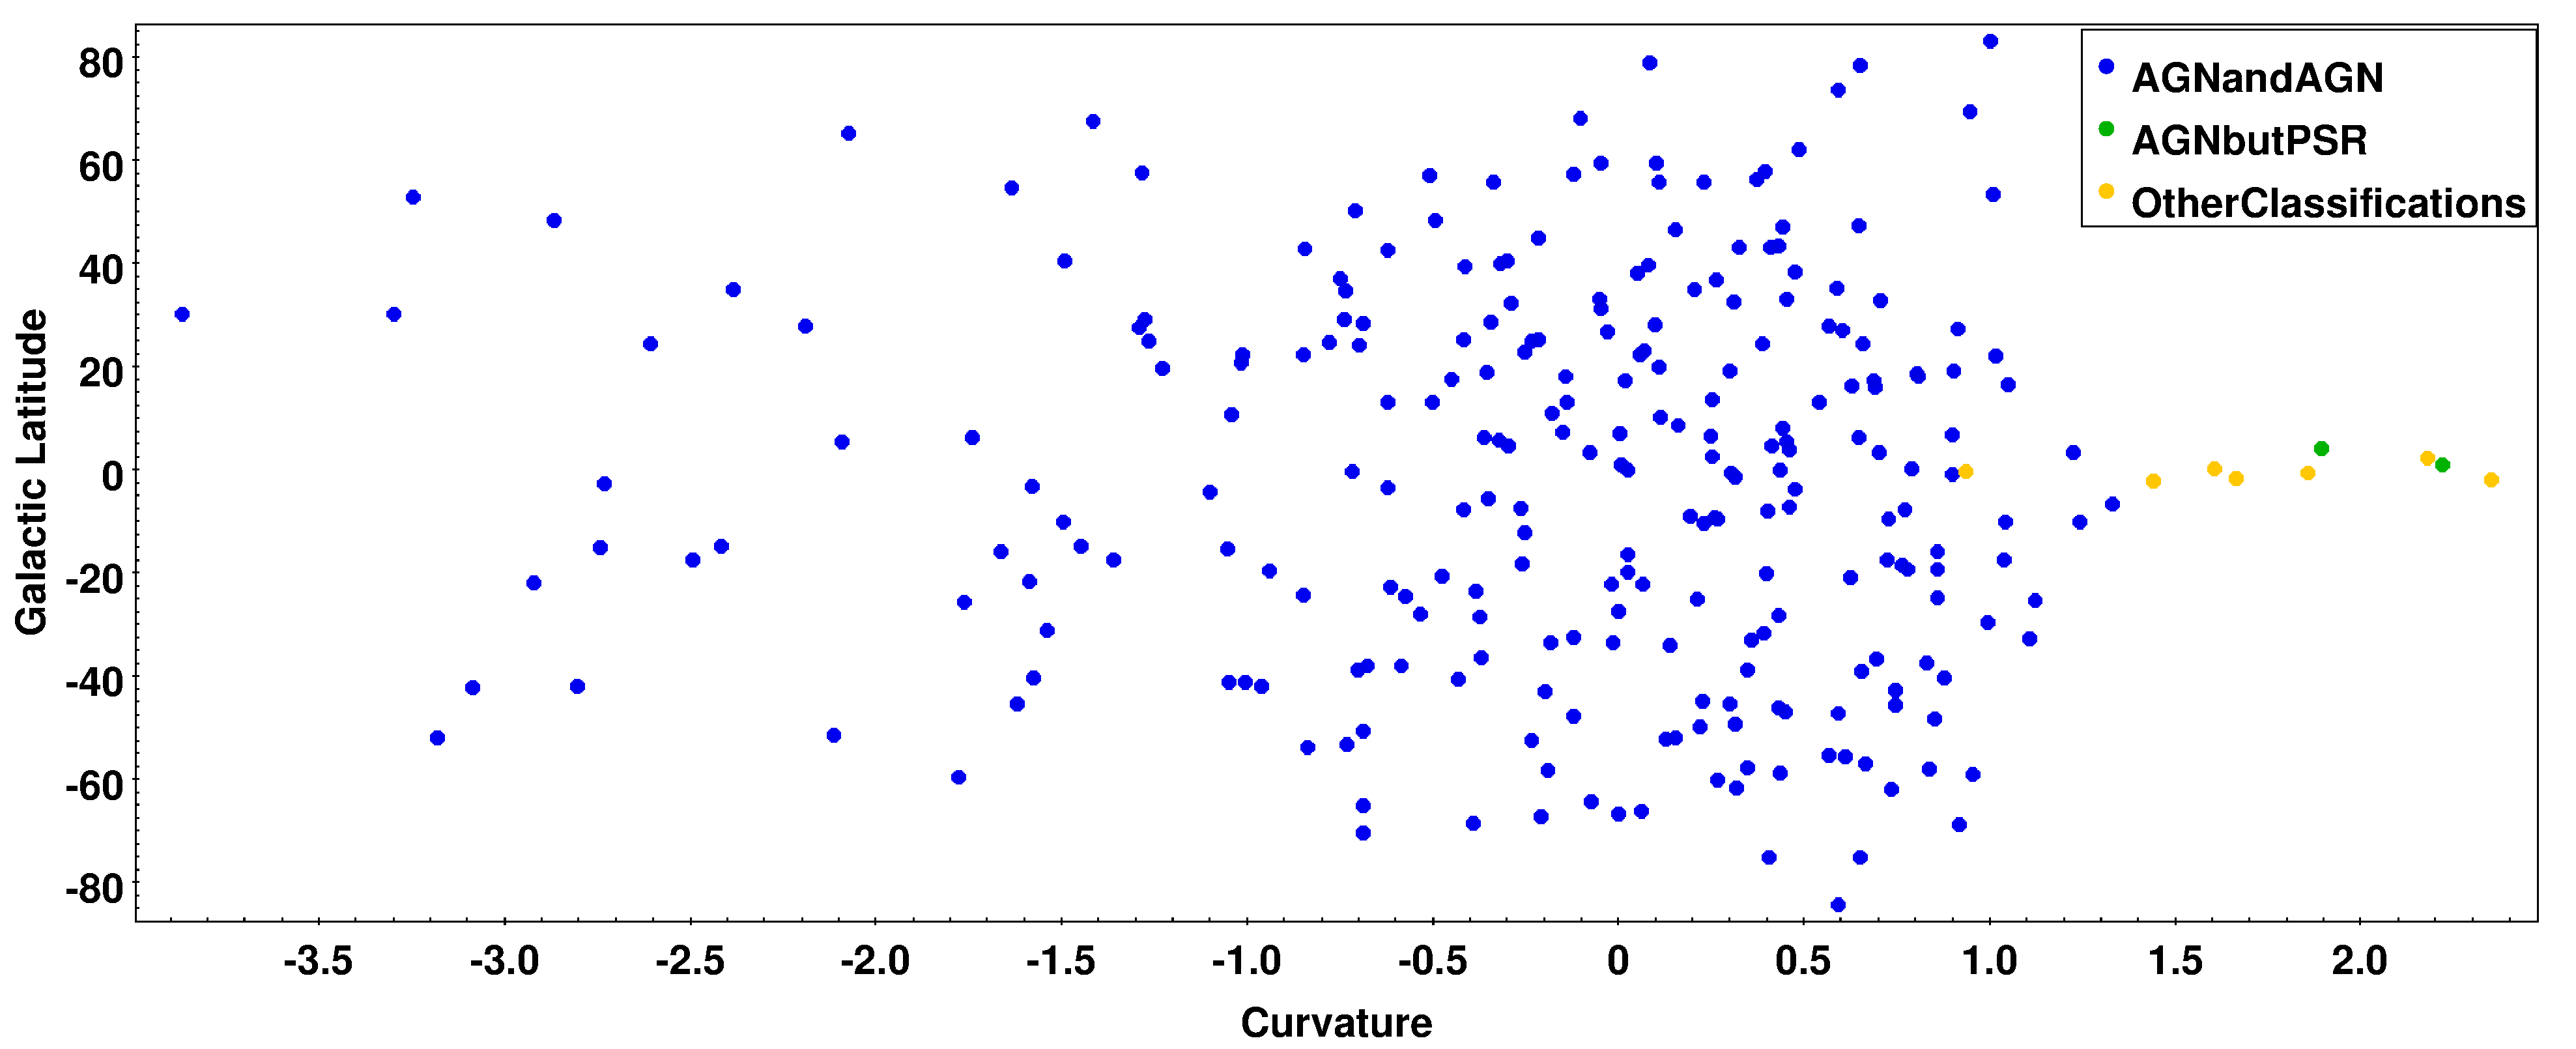
\includegraphics[width=\twopicsp\textwidth]{plots/AGN.pdf}
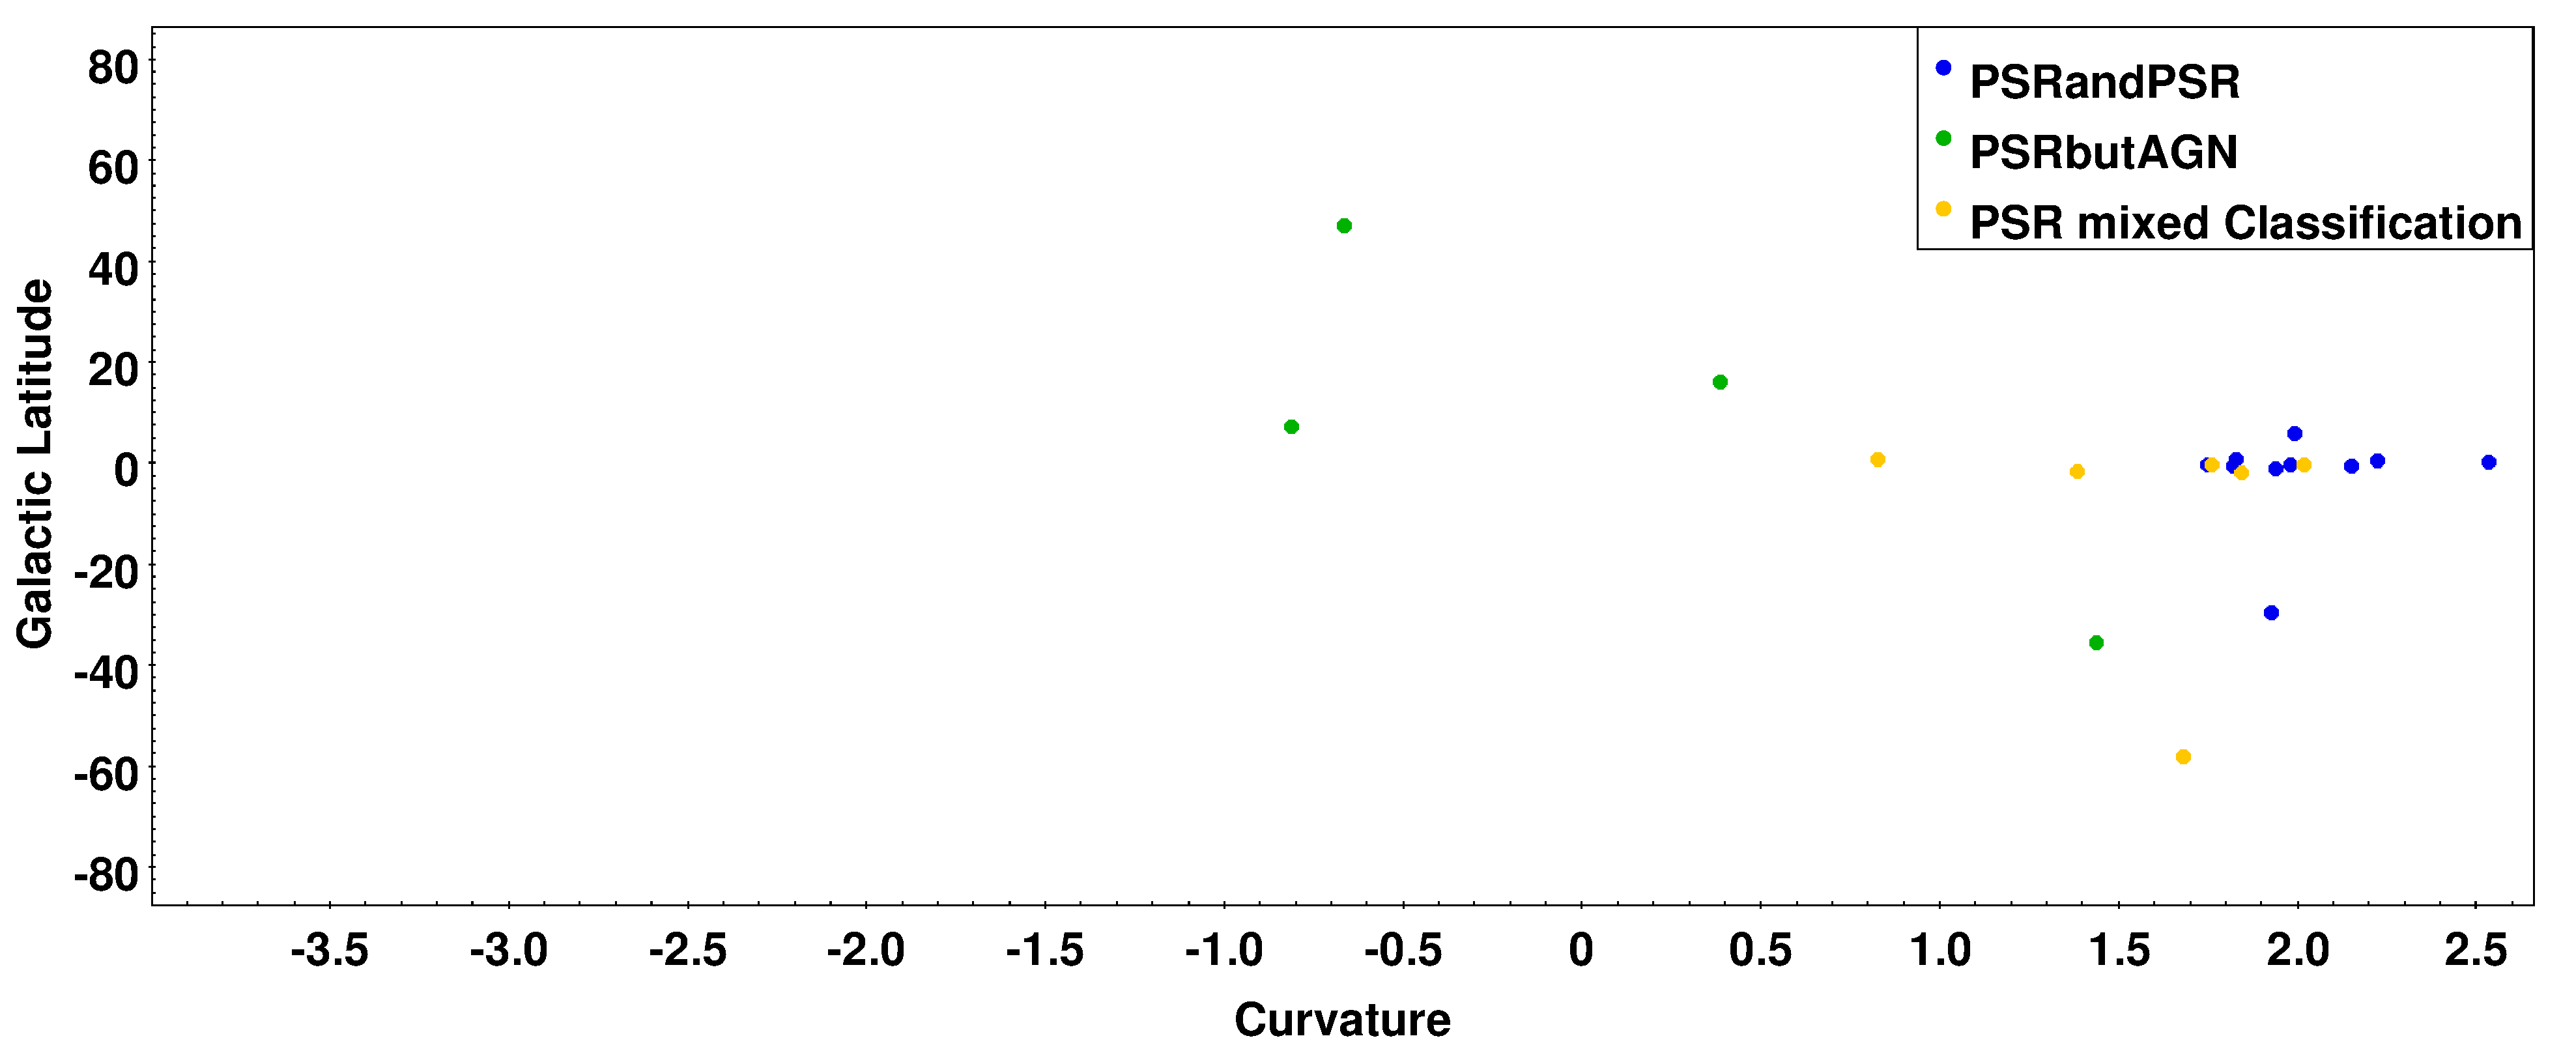
\includegraphics[width=\twopicsp\textwidth]{plots/PSR3.pdf}
\caption{A comparison of the outliers in the test predictions}
=======
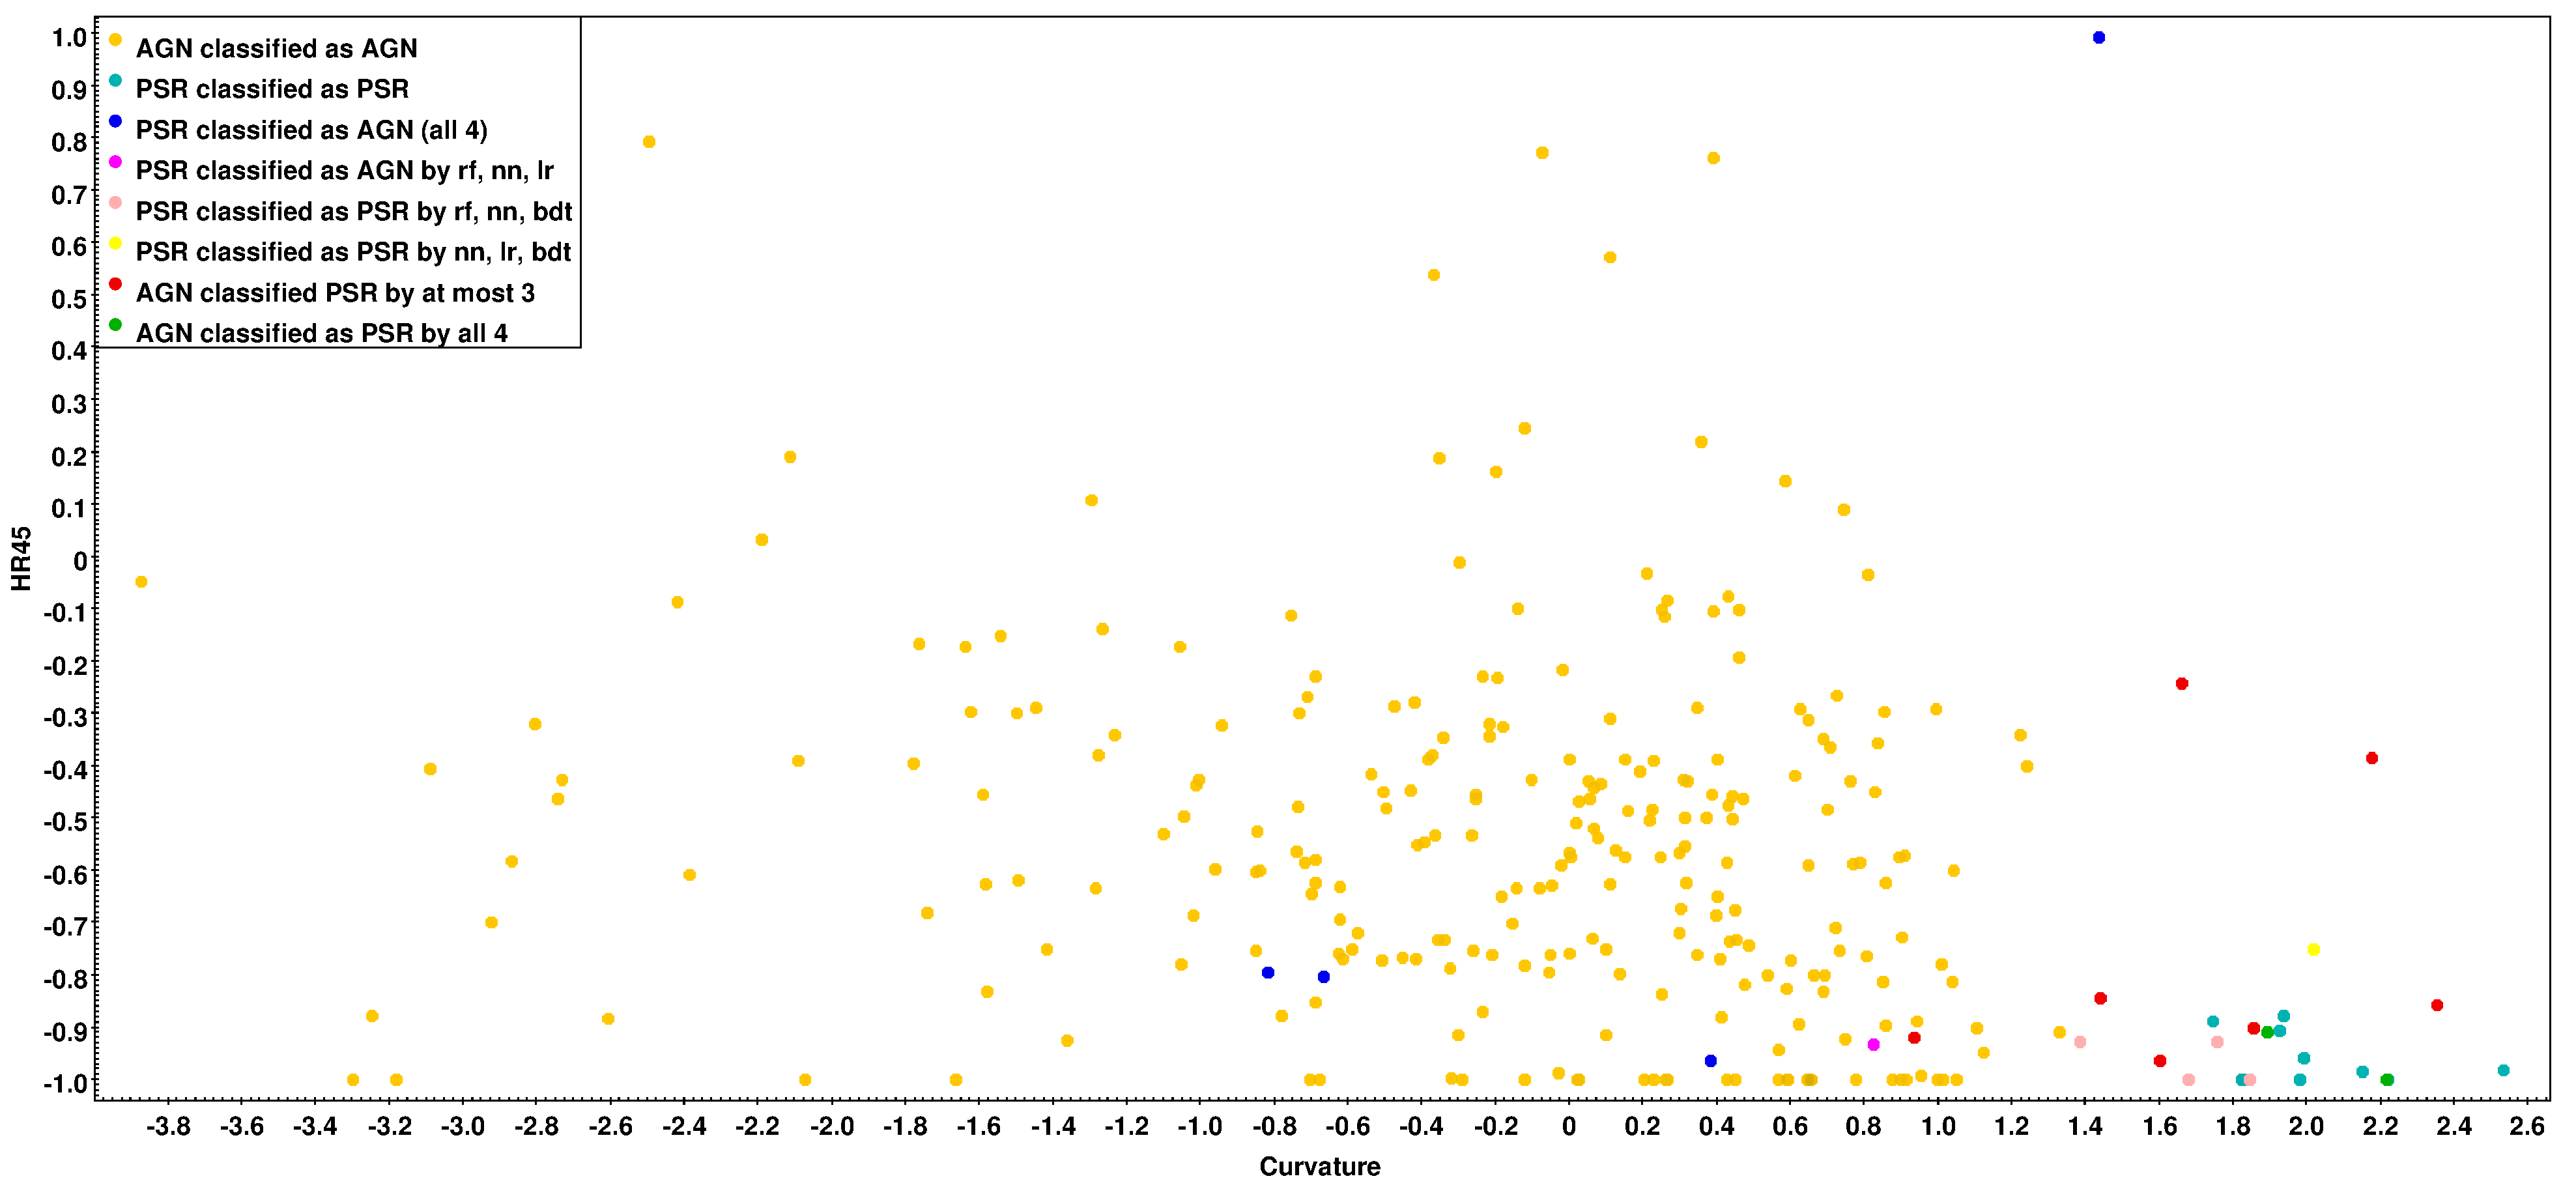
\includegraphics[width=\twopicsp\textwidth]{plots/final_catalog.pdf}
\caption{Comparison of class prediction for unassociated 3FGL sources with classes in 4FGL. 
\dima{Algorithms names in legend should be in capital letters, e.g., NN, RF etc. Different types of dots have similar colors: yellow, cyan. We should use different symbols to make the plot B/W printer friendly.}}
>>>>>>> 5be7c206561412bace1523e8df5da856f811d326
\label{fig:Maps_data}
\end{figure}
